\documentclass{article}\usepackage[]{graphicx}\usepackage[]{color}
%% maxwidth is the original width if it is less than linewidth
%% otherwise use linewidth (to make sure the graphics do not exceed the margin)
\makeatletter
\def\maxwidth{ %
  \ifdim\Gin@nat@width>\linewidth
    \linewidth
  \else
    \Gin@nat@width
  \fi
}
\makeatother

\definecolor{fgcolor}{rgb}{0.345, 0.345, 0.345}
\newcommand{\hlnum}[1]{\textcolor[rgb]{0.686,0.059,0.569}{#1}}%
\newcommand{\hlstr}[1]{\textcolor[rgb]{0.192,0.494,0.8}{#1}}%
\newcommand{\hlcom}[1]{\textcolor[rgb]{0.678,0.584,0.686}{\textit{#1}}}%
\newcommand{\hlopt}[1]{\textcolor[rgb]{0,0,0}{#1}}%
\newcommand{\hlstd}[1]{\textcolor[rgb]{0.345,0.345,0.345}{#1}}%
\newcommand{\hlkwa}[1]{\textcolor[rgb]{0.161,0.373,0.58}{\textbf{#1}}}%
\newcommand{\hlkwb}[1]{\textcolor[rgb]{0.69,0.353,0.396}{#1}}%
\newcommand{\hlkwc}[1]{\textcolor[rgb]{0.333,0.667,0.333}{#1}}%
\newcommand{\hlkwd}[1]{\textcolor[rgb]{0.737,0.353,0.396}{\textbf{#1}}}%

\usepackage{framed}
\makeatletter
\newenvironment{kframe}{%
 \def\at@end@of@kframe{}%
 \ifinner\ifhmode%
  \def\at@end@of@kframe{\end{minipage}}%
  \begin{minipage}{\columnwidth}%
 \fi\fi%
 \def\FrameCommand##1{\hskip\@totalleftmargin \hskip-\fboxsep
 \colorbox{shadecolor}{##1}\hskip-\fboxsep
     % There is no \\@totalrightmargin, so:
     \hskip-\linewidth \hskip-\@totalleftmargin \hskip\columnwidth}%
 \MakeFramed {\advance\hsize-\width
   \@totalleftmargin\z@ \linewidth\hsize
   \@setminipage}}%
 {\par\unskip\endMakeFramed%
 \at@end@of@kframe}
\makeatother

\definecolor{shadecolor}{rgb}{.97, .97, .97}
\definecolor{messagecolor}{rgb}{0, 0, 0}
\definecolor{warningcolor}{rgb}{1, 0, 1}
\definecolor{errorcolor}{rgb}{1, 0, 0}
\newenvironment{knitrout}{}{} % an empty environment to be redefined in TeX

\usepackage{alltt}
%\usepackage[margin=1in]{geometry}   % set up margins
\usepackage[vmargin=1in,hmargin=1in]{geometry}
\usepackage{tikz}
\usepackage{booktabs}
\usepackage{amsmath}
\usepackage[backend=bibtex]{biblatex}


\usepackage{algorithm}
\usepackage{algpseudocode}
\usepackage{pifont}

\thispagestyle{empty}
\begin{center}
\begin{minipage}{1.2\linewidth}
    \centering
 %   \rule{0.4\linewidth}{0.15\linewidth}\par
    \vspace{3cm}
%Thesis title
    \textbf{{\uppercase{\Large Market Basket Analysis in Groceries dataset using R\par}}}
    \vspace{2cm}
    %Degree
    {\Large Business and Data Analytics \par}
    {\textit{\hspace{0.5cm}Project Report} \par}
    \vspace{2cm}
    %University logo
   \hspace{1.9cm} 
\includegraphics[width=0.35\linewidth]{hyderabad-university-publishes-mtech.jpg}\newline
    
    {\textit{\hspace{0.5cm}Submitted by} \par}
%Author's name
  \centering
    {\Large Laltendu Das [15MCMI22]\par}
    {\Large Uma Revathi K N[15MCMI20]\par}
    {\Large  Rosni K V [15MCMI15]\par}
    \vspace{1cm}
    
    %Author's name
    {\textit{\hspace{1cm}Under the Guidance of} \par}
    {\Large Dr. V.Ravi, Professor, IDRBT \par}
    \vspace{2cm}
    \centering
%Date
    {\textbf{\Large November 2015}}
\end{minipage}
\end{center}
\clearpage


\newpage
\renewcommand{\contentsname}{\centering Table of Contents}
\newline
\newline
\tableofcontents
\newpage
%\renewcommand{\listfigurename}{\centering List of Figures}
\listoffigures
%\renewcommand{\listoftables}{\centering List of Tables}
\listoftables
\newpage
\IfFileExists{upquote.sty}{\usepackage{upquote}}{}
\begin{document}
%\SweaveOpts{concordance=TRUE}

%\title {An Attractive Template of a Reproducible Data Analysis Document for an Awesome Class Project}
%\author{Mahbubul Majumder, PhD\\ Department of Mathematics\\ University of Nebraska at Omaha }

%\maketitle



\section{Abstract}
\hspace{0.9cm} Market Basket Analysis is one of the most common and useful types of data analysis for marketing and retailing.  The purpose of market basket analysis is to determine what products customers purchase together.  It takes its name from the idea of customers throwing all their purchases into a shopping cart (a ''market basket") during grocery shopping.  Knowing what products people purchase as a group can be very helpful to a retailer or to any other company.  A store could use this information to place products frequently sold together into the same area, while a catalog or World Wide Web merchant could use it to determine the layout of their catalog and order form.  Direct marketers could use the basket analysis results to determine what new products to offer their prior customers.\par\\
\hspace{0.5cm}There are many ways to see the similarities between items. These are techniques that fall under the general umbrella of association. We consider Association Mining in the groceries dataset. The outcome of this type of technique, in simple terms, is a set of rules that can be understood as ''if this, then that". We then give the description of the Apriori Algorithm  and Frequency Pattern Growth. This study illustrates the use of data mining techniques to construct association rules. Also, it illustrates the rules in a graph. The study also include measures for rule strength using R language.

%\end{abstract}
%\tableofcontents

\section{Introduction} 
\hspace{0.9cm} One of the challenges for companies that have invested heavily in customer data collection is how to extract important information from their vast customer databases and product feature databases, in order to gain competitive advantage. Market basket analysis has been intensively used in many companies as a means to discover product associations and base a retailer’s promotion strategy on them. Market basket analysis is one of the data mining methods focusing on discovering purchasing patterns by extracting associations or co-occurrences from a store’s transactional  data\cite{[1]}.\par\\
\hspace{0.5cm}The input for the market basket analysis is a dataset of purchases. A market basket is 
composed of items bought together in a single trip to a store. The most significant attributes are the transaction identification and item identification. While ignoring the quantity bought and the price. Each transaction represents a purchase, which occurred in a specific time and place. This purchase can be linked to an identified customer(usually carrying a card) or to a non-identified customer.\par\\
\hspace{0.5cm}The dataset with multiple transactions can be shown in a relational table (transaction,item). Corresponding to each attribute there is a set called domain. The table(transaction,item) is a set of all
transactions T=${(T_{1},T_{2},T_{3},....T_{n})}$ where each transaction contain a subset of items $T_{k}={(I_{a},I_{b},I_{c},...)}$\cite{[2]}. Based on the attributes (transaction, item), the market basket will be defined as the N items that are bought together more frequently. Once the market basket with N items is known, we can move on to cross-selling. The next step is to identify all the customers having bought N
-m items of the basket and suggest the purchase of some m missing items. In order to make decisions in marketing, the market basket analysis is a powerful tool supporting the implementation of cross-selling strategies. For instance, if a specific customer's buying profile fits into a identified market basket, the next item will be proposed.\par\\
\hspace{0.5cm}Data mining finds interesting patterns from databases such as association rules, correlations, sequences, classifiers, clusters and many more of which the mining of association rules is one of the most popular problems. Association rule mining finds interesting association or correlation relationships  among a large set of data items. An association rule is a division of each item set into two subset with one subset, the antecedent, thought of as preceding the other subset, the consequent. There are more association rules than there are itemsets. The Apriori algorithm discussed in coming section deals with the large number of rules problem by using selection criteria that reflect the potential utility of association rules.\par
\hspace{0.5cm}Association rules are derived from the frequent itemsets using support and confidence as threshold levels. The interestingness measures like support and confidence plays a vital role in the association analysis. The support is defined as percentage of transactions that contained in the rule and is given by\\\\
Support = ($\#$ of transactions involving A and B) / (total number of transactions).\\\\
The other factor is confidence it is the percentage of transactions that contain B if they contain A.\\\\
Confidence = Probability (B if A) = P({B / A})\\\\
Confidence = {($\#$ of transactions involving A and B) / (total number of transactions that have A)}.\par
\hspace{0.5cm}Item sets that satisfy minimum support and minimum confidence are called strong association rule. For this study we used groceries dataset which contains: a collection of receipts with each line representing 1 receipt and the items purchased.\par
\hspace{0.5cm} Although the Apriori algorithm processes data in a  different manner from the algorithms 
FPGrowth and Create Association Rules, gives a lot of insight about our data. A major advantage of  the  algorithm FP Growth compared to others of the same type is the fact that it uses only two scans of the data and it can be applied to larger data sets. The frequent sets of articles are searched for positive entries from the data base. The entry data set must contain only bionominal attributes. If the data contains other types of attributes preprocessing operators must be used to transform the data set. In RapidMiner the process of exploitation of frequent sets is divided into two parts, first are generated all frequent sets of articles after which are generated the association rules from the frequent sets. 
\section{Algorithm Description}
\subsection{Apriori Algorithm}\hspace{0.9cm}Apriori is a seminal algorithm proposed by R. Agrawal and R. Srikant in 1994 for mining frequent itemsets for Boolean association rules. It takes all of the transactions in the database into account in order to define the market basket. The market basket can be represented with association rules, with a left and a right side Left $\implies$ Right. For instance, given an itemset $\{A,B,C \}$ the rule $\{B,C \} \implies \{A \}$ should be read as follows if a customer bought $\{ B,C \}$ he would probably buy $\{A \}$.\par\\
\hspace{0.5cm}The name of the algorithm is based on the fact that the algorithm uses prior knowledge of frequent itemset properties. Apriori employs an iterative approach known as a level-wise search, where k-itemsets are used to explore (k + 1)-itemsets. First, the set of frequent 1-itemsets is found by scanning the database to accumulate the count for each item, and collecting those items that satisfy minimum support. The resulting set is denoted $L_{1}$. Next,$L_{1}$ is used to find $L_{2}$, the set of frequent 2-itemsets, which is used to find $L_{3}$ , and so on, until no more frequent k-itemsets can be found. The finding of each $L_{k}$ requires one full scan of the database.To improve the efficiency of the level-wise generation of frequent itemsets, an important property called the Apriori property, explained below, is used to reduce the search space.\cite{[3]}\\
\textbf{Apriori property :}\textit{All nonempty subsets of a frequent itemset must also be frequent.}\par\\
\hspace{0.5cm}The Apriori property is based on the following observation. By definition, if an itemset
I does not satisfy the minimum support threshold, $min\_sup$, then I is not frequent; that
is,$P(I) < min\_sup$. If an item A is added to the itemset I, then the resulting itemset (i.e.,$I\bigcup A$) cannot occur more frequently than I. Therefore, I $\bigcup$ A is not frequent either; that is,$P(I \bigcup A) < min\_sup$.\par\\
\hspace{0.5cm}This property belongs to a special category of properties called antimonotone in the
sense that \textit{if a set cannot pass a test, all of its supersets will fail the same test as well}. It is called \textit{antimonotone} because the property is monotonic in the context of failing a test. The algorithm pseudo code is given below.\par\\

\begin{algorithm}
\caption{Apriori algorithm}
\label{CHalgorithm}
\begin{algorithmic}[1]
\Procedure{Apriori\textendash($in \hspace{0.1cm}D$ : $transactional\hspace{0.1cm} Database$ ; $minsup$: $minimum\hspace{0.1cm}support$)}{}
%\For{each node $i$ \Pisymbol{psy}{206} $N$ }
\State $L_1$=$\{Large 1- itemsets\}$
\State k=2
\While{ ( L_{k-1}$\neq\phi$) }
\State $C_k$=apriori$\_gen(L_{k-1})$ 
\For {all transactions \textit{t} in D}
\State $C^t=subset(C_k,t)$
\For {all candidates $c \in C^t$}
\State c.count=c.count+1
\EndFor
\EndFor
\EndWhile  
\State {$L_k$=$\{$ c $\in$ $C_k$ $\vbar$ c.count $\geq$ minsup $\}$}
\Comment{Second Pruning Step}
\State{k=k+1}
%\State let $k$ \Pisymbol{psy}{206} $N1$ ($i$) U {$i$} be s.t
%\State QOS($k$) = max {QOS($j$) \textbar $j$ \Pisymbol{psy}{206} $N1$($i$)  U $i$}
%\State MPRSet($i$) = $k$
%\EndFor
\EndProcedure
\Procedure{apriori$\_gen$($L_{k-1}$)}{}
\State $C_k$=$\phi$
\For{all itemsets X $\in$ $L_{k-1}$ and Y $\in$ $L_{k-1}$}
\If{$X_1$=$Y_1$ $\wedge$ ....$\wedge$ $X_{k-2}$=$Y_{k-2}$ $\wedge$ $X_{k-1}$ $<$ $Y_{k-1}$ }
\State{C=$X_1$$X_2$...$X_{k-1}$$Y_{k-1}$}
\State{add C to $C_k$}
\EndIf
\Comment{First Pruning Step}
\EndFor
\State {Delete candidates itemsets in $C_k$ whose any subset is not in $L_{k-1}$}
\EndProcedure
\end{algorithmic}
\end{algorithm}
\hspace{0.5cm} Step 2 generates 1-itemsets, i.e., the frequent items. These 1-itemsets are stored in $L_1$ list, which will be used to generate $C_2$. $C_2$ is the list of the candidate 2-itemsets. The generationoperation of $C_{k+1}$ from $L_k$ is done by $apriori\_gen$ algorithm. $Apriori\_gen$ takes two different last items k-itemsets to generate candidate (k+1)-itemset by joining the similar k-1 items with the last
different items. For example, let X and Y are two frequent 3-itemsets in $L_3$, such that X=abc and Y=abd
, then the generated candidate 4-itemset is abcd which will be added to $C_4$ list.\par\\
\hspace{0.5cm}$Apriori\_gen$ performs the first complex pruning step to exclude infrequent candidates. This is done in step 24. It degenerates the generated candidate (k+1)-itemset to its k-itemset subsets. If there is any subset not member in $L_k$, then its candidate will be removed from $C_{k+1}$. Steps 7 to 10 are responsible for the second pruning step. The core of these steps is the function subset that checks the subsetness of a candidate in a transaction. Subset function depends on a hash tree, which has been built gradually during the progress of mining the large itemsets in each iteration.\par\\
\hspace{0.5cm}The outputs of the Apriori algorithm are easy to understand and many new patterns can be identified. However, the sheer number of association rules may make the interpretation of the results difficult. A second weakness of the algorithm is the computational times when it searches for large itemsets, due to the exponential complexity of the algorithm. Figure[1] provides a high-level illustration of the frequent itemset generation part of the Apriori algorithm for the transactions shown in Table [1]\\
\begin{table}[t]
\caption{Transactions}
\centering
\begin{tabular}{c|c}
\toprule
TID & Items \\
\midrule
1 & $\{$ Bread, Milk $\}$\\
2 & $\{$ Bread, Diapers, Beer, Eggs $\}$\\
3 & $\{$ Milk, Diapers, Beer, Cola $\}$\\
4 & $\{$ Bread, Milk, Diapers, Beer $\}$\\
5 & $\{$ Bread, Milk, Diapers, Cola $\}$\\
\bottomrule
\end{tabular}
\label{tab2}
\end{table}

\begin{figure}[h]
\begin{center}
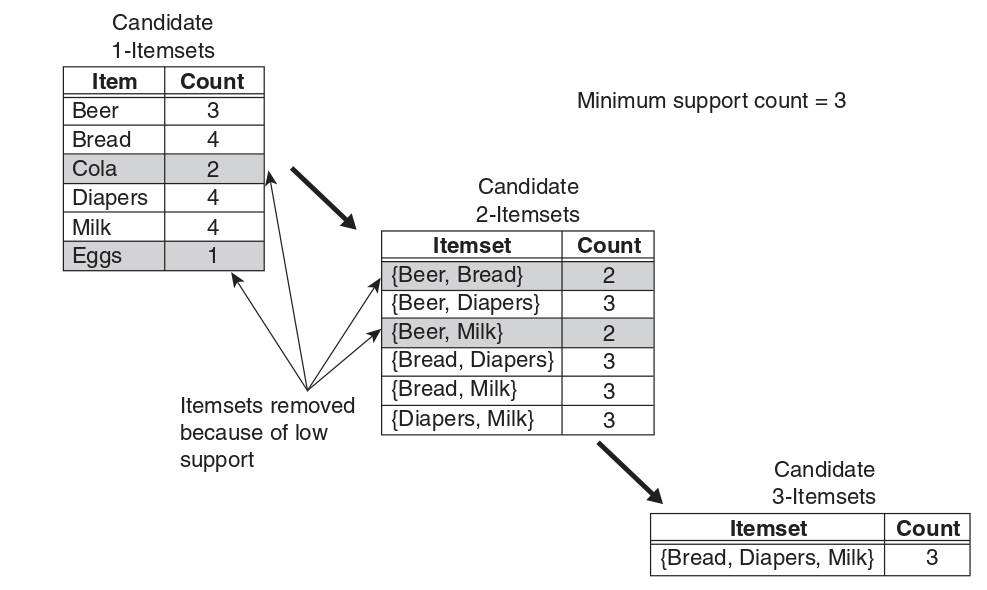
\includegraphics [scale=0.35]{apriori.png}
\end{center}
\caption{Illustration of frequent itemset generation using the Apriori algorithm.}
\end{figure}
\subsection{FP  Growth  algorithm  for  frequent  pattern generation}\hspace{0.9cm}An interesting method to frequent pattern mining without generating candidate pattern is called frequent-pattern growth, or simply FP-growth, which adopts a divide-and-conquer strategy. First, it compresses the database representing frequent items into a frequent-pattern tree, or FP-tree, which retains the itemset association information. It then divides the compressed database into a set of conditional databases (a special kind of projected database), each associated with one frequent item or pattern fragment, and mines each such database separately\cite{[7]}.\par\\
\hspace{0.5cm}It overcomes the two major problems of Apriori algorithm. As in Apriori algorithm.\\
%\begin{enumerate}
1. It do not generates large number of candidate items. \\
2. No repeated scan of original database is required. \\
%\end{enumerate}
\subsubsection{FP-Tree Representation}\hspace{0.9cm}An FP-tree is a compressed representation of the input data. It is constructed by reading the data set one transaction at a time and mapping each transaction onto a path in the FP-tree.  As different transactions can have several items in common, their paths may overlap. The more the paths overlap with one another, the more compression we can achieve using the FP-tree structure. If
the size of the FP-tree is small enough to fit into main memory, this will allow us to extract frequent itemsets directly from the structure in memory instead of making repeated passes over the data stored on disk.\par
\begin{figure}[h]
\begin{center}
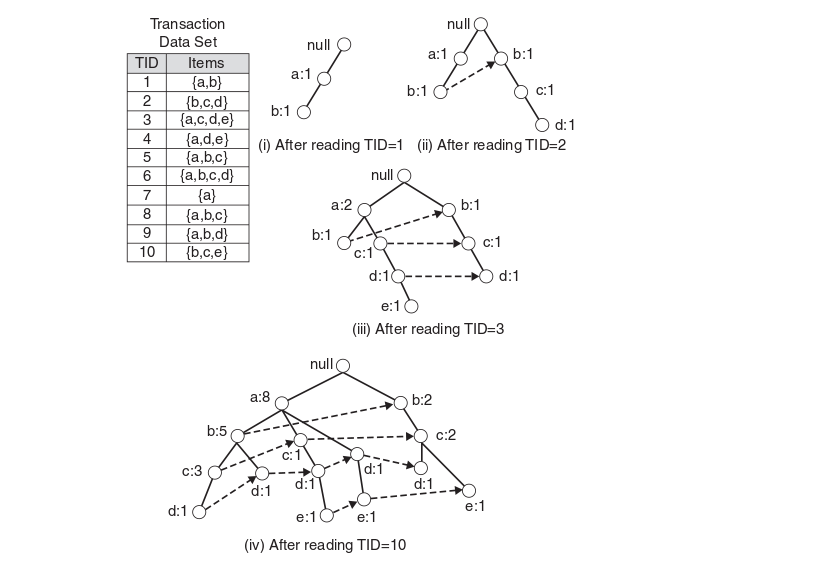
\includegraphics [scale=0.60]{fpeg.png}
\end{center}
\caption{contruction of an fp tree}
\end{figure}
\hspace{0.5cm}Figure[2] shows a data set that contains ten transactions and five items. The structures of the FP-tree after reading the first three transactions are also depicted in the diagram. Each node in the tree contains the label of an item along with a counter that shows the number of transactions mapped onto the given path. Initially, the FP-tree contains only the root node represented by the null symbol. The FP-tree is subsequently extended in the following way:
\begin{itemize}
\item The data set is scanned once to determine the support count of each item. Infrequent items are discarded, while the frequent items are sorted in decreasing support counts. For the data set shown in Figure [2], a is the most frequent item, followed by b,c,d, and e.
\item The algorithm makes a second pass over the data to construct the FP-tree. After reading the first transaction,$\{$ a, b$\}$, the nodes labeled as a and b are created. A path is then formed from \textit{null} $\implies$ a $\implies$ b to encode the transaction. Every node along the path has a frequency count of 1.
\item After reading the second transaction,$\{$ b,c,d$\}$ , a new set of nodes is created for items b ,
c,and d. A path is then formed to represent the transaction by connecting the nodes \textit{null} $\implies$ b $\implies$ c $\implies$ d. Every node along this path also has a frequency count equal to one. Although the first two transactions have an item in common, which is b, their paths are disjoint because the transactions do not share a common prefix.
\item The third transaction,$\{$ a, c, d, e $\}$, shares a common prefix item (which is a) with the first transaction. As a result, the path for the third transaction, \textit{null} $\implies$ a $\implies$ c $\implies$ d $\implies$ e, overlaps with the path for the first transaction, \textit{null} $\implies$ a $\implies$ b. Because of their overlapping path, the frequency count for node a is incremented to two, while the frequency counts for the newly created nodes, c, d, and e, are equal to one.
\item This process continues until every transaction has been mapped onto one of the paths given in the FP-tree. The resulting FP-tree after reading all the transactions is shown at the bottom of Figure [2].
\end{itemize}
\subsubsection{Frequent Itemset Generation in FP-Growth Algorithm}\hspace{0.9cm}FP-growth is an algorithm that generates frequent itemsets from an FP-tree by exploring the tree in a bottom-up fashion. The algorithm pseudo code is given below. FP-growth is an interesting algorithm because it illustrates how a compact representation of the transaction data set helps to efficiently generate frequent itemsets. In addition, for certain transaction data sets, FP-growth outperforms the standard Apriori algorithm by several orders of magnitude. The run time performance of FP-growth depends on the compaction factor of the data set. If the resulting conditional FP-trees are very bushy (in the worst case, a full prefix tree), then the performance of the algorithm degrades significantly because it has to generate a large number of subproblems and merge the results returned by each subproblem.\\
\begin{algorithm}
\caption{Algorithm FP-growth}
\label{CHalgorithm}
\begin{algorithmic}[1]
\Procedure{FP-growth\textendash($Tree, \hspace{0.1cm}$\alpha$)}{}
\If{Tree contains a single path P }
\For {each combination (denoted as $\beta$) of the node in the path P}
\State generate pattern $\beta$ $\bigcup$ $\alpha$ with $support\_count$ = minimum support count of nodes in $\beta$;
\EndFor
\Else
\For{each $a_{i}$ in the header of Tree}
\State generate pattern $\beta$= $a_{i}$ $\bigcup$ $\alpha$ with $support\_count$=$a_{i}$.$support\_count$;
\State construct $\beta$'s conditional pattern base and then $\beta$'s conditional $FP\_tree$ $Tree_{\beta}$;
\If{$Tree_{\beta}$ $\neq$ $\phi$ }
\State call $FP\_growth($Tree_{\beta}$,$\beta$);
\EndIf
\EndFor
\EndProcedure
\end{algorithmic}
\end{algorithm}

\section{Data set description}\hspace{0.9cm}The Groceries data set we used for this study contains 1 month (30 days) of real-world point-of-sale transaction data from a typical local grocery outlet. The data set is provided by Michael Hahsler, Kurt Hornik and Thomas Reutterer\cite{[3]}. The packages \textit{arules} and \textit{arulesViz} are used here for association mining tasks.\\
\begin{knitrout}
\definecolor{shadecolor}{rgb}{0.969, 0.969, 0.969}\color{fgcolor}\begin{kframe}
\begin{alltt}
\hlkwd{library}\hlstd{(arules)}
\hlkwd{library}\hlstd{(arulesViz)}
\hlstd{groceries} \hlkwb{<-} \hlkwd{read.transactions}\hlstd{(}\hlstr{"/home/freestyler/BDA_project2/groceries.csv"}\hlstd{,} \hlkwc{sep} \hlstd{=} \hlstr{","}\hlstd{)}
\end{alltt}
\end{kframe}
\end{knitrout}
\par We can see how the items are organized in the dataset by inspect method. The data set contains 9835 transactions and the items are aggregated to 169 categories. \\
\begin{knitrout}
\definecolor{shadecolor}{rgb}{0.969, 0.969, 0.969}\color{fgcolor}\begin{kframe}
\begin{alltt}
\hlkwd{inspect}\hlstd{(groceries[}\hlnum{1}\hlopt{:}\hlnum{2}\hlstd{])}
\end{alltt}
\begin{verbatim}
##   items                
## 1 {citrus fruit,       
##    margarine,          
##    ready soups,        
##    semi-finished bread}
## 2 {coffee,             
##    tropical fruit,     
##    yogurt}
\end{verbatim}
\begin{alltt}
\hlkwd{print}\hlstd{(}\hlkwd{dim}\hlstd{(groceries))}
\end{alltt}
\begin{verbatim}
## [1] 9835  169
\end{verbatim}
\end{kframe}
\end{knitrout}
The summary of the groceries dataset is given by:
\begin{knitrout}
\definecolor{shadecolor}{rgb}{0.969, 0.969, 0.969}\color{fgcolor}\begin{kframe}
\begin{alltt}
\hlkwd{summary}\hlstd{(groceries)}
\end{alltt}
\begin{verbatim}
## transactions as itemMatrix in sparse format with
##  9835 rows (elements/itemsets/transactions) and
##  169 columns (items) and a density of 0.02609146 
## 
## most frequent items:
##       whole milk other vegetables       rolls/buns             soda 
##             2513             1903             1809             1715 
##           yogurt          (Other) 
##             1372            34055 
## 
## element (itemset/transaction) length distribution:
## sizes
##    1    2    3    4    5    6    7    8    9   10   11   12   13   14   15 
## 2159 1643 1299 1005  855  645  545  438  350  246  182  117   78   77   55 
##   16   17   18   19   20   21   22   23   24   26   27   28   29   32 
##   46   29   14   14    9   11    4    6    1    1    1    1    3    1 
## 
##    Min. 1st Qu.  Median    Mean 3rd Qu.    Max. 
##   1.000   2.000   3.000   4.409   6.000  32.000 
## 
## includes extended item information - examples:
##             labels
## 1 abrasive cleaner
## 2 artif. sweetener
## 3   baby cosmetics
\end{verbatim}
\end{kframe}
\end{knitrout}

we can visualize each item with support greater than 0.025 shown in Figure [3].
\begin{knitrout}
\definecolor{shadecolor}{rgb}{0.969, 0.969, 0.969}\color{fgcolor}\begin{kframe}
\begin{alltt}
\hlkwd{itemFrequencyPlot}\hlstd{(groceries,}\hlkwc{support}\hlstd{=}\hlnum{0.025}\hlstd{,}\hlkwc{cex.names}\hlstd{=}\hlnum{0.8}\hlstd{,}\hlkwc{xlim}\hlstd{=}\hlkwd{c}\hlstd{(}\hlnum{0}\hlstd{,}\hlnum{0.3}\hlstd{),}\hlkwc{type}\hlstd{=}\hlstr{"relative"}\hlstd{,}
                  \hlkwc{horiz}\hlstd{=}\hlnum{TRUE}\hlstd{,}\hlkwc{col}\hlstd{=}\hlstr{"dark red"}\hlstd{,}\hlkwc{las}\hlstd{=}\hlnum{1}\hlstd{,}\hlkwc{xlab}\hlstd{=}\hlkwd{paste}\hlstd{(}\hlstr{"Proportions of Market 
                  Baskets containing Item"}\hlstd{,}\hlstr{"\textbackslash{}n(Item Relative Frequency or Support)"}\hlstd{))}
\end{alltt}
\end{kframe}\begin{figure}
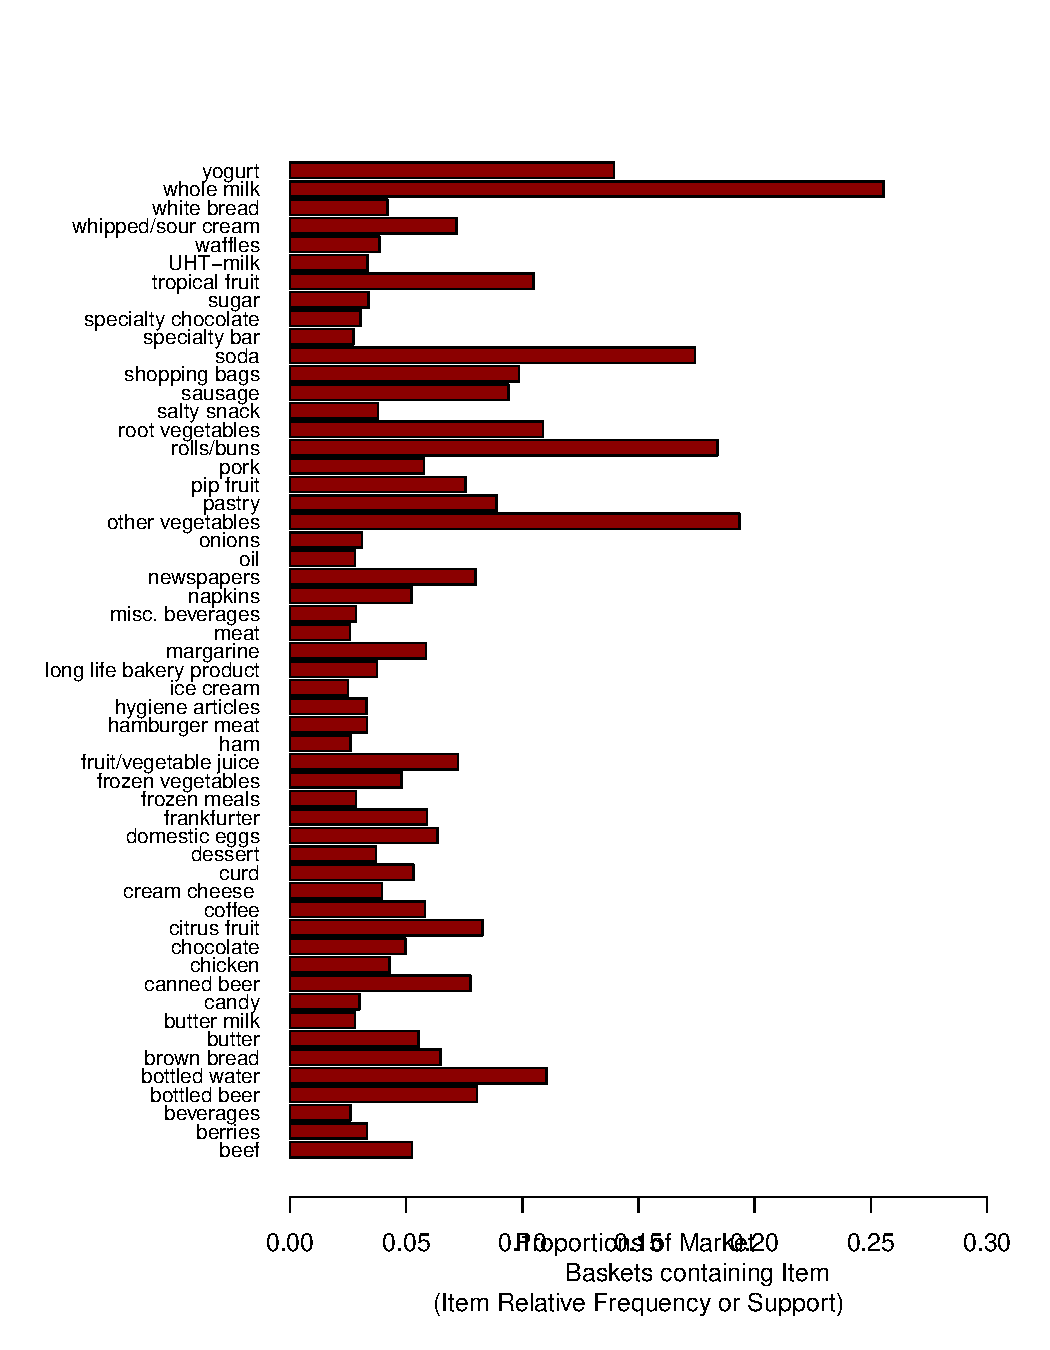
\includegraphics[width=\maxwidth]{figure/unnamed-chunk-5-1} \caption[Item frequency]{Item frequency}\label{fig:unnamed-chunk-5}
\end{figure}


\end{knitrout}
\section{Result and Discussions}
\subsection{Apriori algorithm}\hspace{0.9cm}To mine the rules, we have to pass the minimum required support and confidence. We set the minimum support to 0.001; Support is the fraction of which our item set occurs in our dataset. We set the minimum confidence of 0.8 ;Confidence is the probability that a rule is correct for a new transaction with items on the left. Lift is another measure, the ratio by which by the confidence of a rule exceeds the expected confidence. If the lift is 1 it indicates that the items on the left and right are independent.\par
\begin{knitrout}
\definecolor{shadecolor}{rgb}{0.969, 0.969, 0.969}\color{fgcolor}\begin{kframe}
\begin{alltt}
\hlstd{rules} \hlkwb{=} \hlkwd{apriori}\hlstd{(groceries,} \hlkwc{parameter}\hlstd{=}\hlkwd{list}\hlstd{(}\hlkwc{support}\hlstd{=}\hlnum{0.001}\hlstd{,} \hlkwc{confidence}\hlstd{=}\hlnum{0.8}\hlstd{))}
\end{alltt}
\begin{verbatim}
## 
## parameter specification:
##  confidence minval smax arem  aval originalSupport support minlen maxlen
##         0.8    0.1    1 none FALSE            TRUE   0.001      1     10
##  target   ext
##   rules FALSE
## 
## algorithmic control:
##  filter tree heap memopt load sort verbose
##     0.1 TRUE TRUE  FALSE TRUE    2    TRUE
## 
## apriori - find association rules with the apriori algorithm
## version 4.21 (2004.05.09)        (c) 1996-2004   Christian Borgelt
## set item appearances ...[0 item(s)] done [0.00s].
## set transactions ...[169 item(s), 9835 transaction(s)] done [0.01s].
## sorting and recoding items ... [157 item(s)] done [0.00s].
## creating transaction tree ... done [0.01s].
## checking subsets of size 1 2 3 4 5 6 done [0.02s].
## writing ... [410 rule(s)] done [0.00s].
## creating S4 object  ... done [0.00s].
\end{verbatim}
\begin{alltt}
\hlstd{rules}\hlkwb{<-}\hlkwd{sort}\hlstd{(rules,} \hlkwc{by}\hlstd{=}\hlstr{"lift"}\hlstd{,} \hlkwc{decreasing}\hlstd{=}\hlnum{TRUE}\hlstd{)}
\end{alltt}
\end{kframe}
\end{knitrout}
Sometimes, rules will repeat. Eliminate the redundant rules by:
\begin{knitrout}
\definecolor{shadecolor}{rgb}{0.969, 0.969, 0.969}\color{fgcolor}\begin{kframe}
\begin{alltt}
\hlstd{subset.matrix} \hlkwb{<-} \hlkwd{is.subset}\hlstd{(rules, rules)}
\hlstd{subset.matrix[}\hlkwd{lower.tri}\hlstd{(subset.matrix,} \hlkwc{diag}\hlstd{=T)]} \hlkwb{<-} \hlnum{NA}
\hlstd{redundant} \hlkwb{<-} \hlkwd{colSums}\hlstd{(subset.matrix,} \hlkwc{na.rm}\hlstd{=T)} \hlopt{>=} \hlnum{1}
\hlstd{rules.pruned} \hlkwb{<-} \hlstd{rules[}\hlopt{!}\hlstd{redundant]}
\hlstd{rules}\hlkwb{<-}\hlstd{rules.pruned}
\end{alltt}
\end{kframe}
\end{knitrout}
As a result the number of rules reduced from 410 to 370. 
\begin{knitrout}
\definecolor{shadecolor}{rgb}{0.969, 0.969, 0.969}\color{fgcolor}\begin{kframe}
\begin{alltt}
\hlkwd{summary}\hlstd{(rules)}
\end{alltt}
\begin{verbatim}
## set of 370 rules
## 
## rule length distribution (lhs + rhs):sizes
##   3   4   5   6 
##  29 226 111   4 
## 
##    Min. 1st Qu.  Median    Mean 3rd Qu.    Max. 
##   3.000   4.000   4.000   4.243   5.000   6.000 
## 
## summary of quality measures:
##     support           confidence          lift       
##  Min.   :0.001017   Min.   :0.8000   Min.   : 3.131  
##  1st Qu.:0.001017   1st Qu.:0.8333   1st Qu.: 3.312  
##  Median :0.001220   Median :0.8462   Median : 3.588  
##  Mean   :0.001257   Mean   :0.8659   Mean   : 3.974  
##  3rd Qu.:0.001322   3rd Qu.:0.9091   3rd Qu.: 4.373  
##  Max.   :0.003152   Max.   :1.0000   Max.   :11.235  
## 
## mining info:
##       data ntransactions support confidence
##  groceries          9835   0.001        0.8
\end{verbatim}
\begin{alltt}
\hlkwd{options}\hlstd{(}\hlkwc{digits}\hlstd{=}\hlnum{2}\hlstd{)}
\hlkwd{inspect}\hlstd{(rules[}\hlnum{1}\hlopt{:}\hlnum{15}\hlstd{])}
\end{alltt}
\begin{verbatim}
##    lhs                        rhs               support confidence lift
## 1  {liquor,                                                            
##     red/blush wine}        => {bottled beer}     0.0019       0.90 11.2
## 2  {citrus fruit,                                                      
##     fruit/vegetable juice,                                             
##     other vegetables,                                                  
##     soda}                  => {root vegetables}  0.0010       0.91  8.3
## 3  {oil,                                                               
##     other vegetables,                                                  
##     tropical fruit,                                                    
##     whole milk,                                                        
##     yogurt}                => {root vegetables}  0.0010       0.91  8.3
## 4  {citrus fruit,                                                      
##     fruit/vegetable juice,                                             
##     grapes}                => {tropical fruit}   0.0011       0.85  8.1
## 5  {other vegetables,                                                  
##     rice,                                                              
##     whole milk,                                                        
##     yogurt}                => {root vegetables}  0.0013       0.87  8.0
## 6  {oil,                                                               
##     other vegetables,                                                  
##     tropical fruit,                                                    
##     whole milk}            => {root vegetables}  0.0013       0.87  8.0
## 7  {ham,                                                               
##     other vegetables,                                                  
##     pip fruit,                                                         
##     yogurt}                => {tropical fruit}   0.0010       0.83  7.9
## 8  {beef,                                                              
##     citrus fruit,                                                      
##     other vegetables,                                                  
##     tropical fruit}        => {root vegetables}  0.0010       0.83  7.6
## 9  {butter,                                                            
##     cream cheese ,                                                     
##     root vegetables}       => {yogurt}           0.0010       0.91  6.5
## 10 {butter,                                                            
##     sliced cheese,                                                     
##     tropical fruit,                                                    
##     whole milk}            => {yogurt}           0.0010       0.91  6.5
## 11 {cream cheese ,                                                     
##     curd,                                                              
##     other vegetables,                                                  
##     whipped/sour cream}    => {yogurt}           0.0010       0.91  6.5
## 12 {butter,                                                            
##     other vegetables,                                                  
##     tropical fruit,                                                    
##     white bread}           => {yogurt}           0.0010       0.91  6.5
## 13 {pip fruit,                                                         
##     sausage,                                                           
##     sliced cheese}         => {yogurt}           0.0012       0.86  6.1
## 14 {butter,                                                            
##     curd,                                                              
##     tropical fruit,                                                    
##     whole milk}            => {yogurt}           0.0012       0.86  6.1
## 15 {butter,                                                            
##     tropical fruit,                                                    
##     white bread}           => {yogurt}           0.0011       0.85  6.1
\end{verbatim}
\end{kframe}
\end{knitrout}
Now we can target items to generate rules. For example, there are two types of targets that we are interested with an example of ``whole milk".\\
1.What are customers likely to buy before buying whole milk\\
2.What are customers likely to buy if they purchase whole milk$\?$\\
For that we can adjust our apriori function as follows:
\begin{knitrout}
\definecolor{shadecolor}{rgb}{0.969, 0.969, 0.969}\color{fgcolor}\begin{kframe}
\begin{alltt}
\hlstd{rules1}\hlkwb{<-}\hlkwd{apriori}\hlstd{(}\hlkwc{data}\hlstd{=groceries,} \hlkwc{parameter}\hlstd{=}\hlkwd{list}\hlstd{(}\hlkwc{supp}\hlstd{=}\hlnum{0.001}\hlstd{,}\hlkwc{conf} \hlstd{=} \hlnum{0.08}\hlstd{),}
               \hlkwc{appearance} \hlstd{=} \hlkwd{list}\hlstd{(}\hlkwc{default}\hlstd{=}\hlstr{"lhs"}\hlstd{,}\hlkwc{rhs}\hlstd{=}\hlstr{"whole milk"}\hlstd{),}
               \hlkwc{control} \hlstd{=} \hlkwd{list}\hlstd{(}\hlkwc{verbose}\hlstd{=F))}
\hlstd{rules1}\hlkwb{<-}\hlkwd{sort}\hlstd{(rules1,} \hlkwc{decreasing}\hlstd{=}\hlnum{TRUE}\hlstd{,}\hlkwc{by}\hlstd{=}\hlstr{"lift"}\hlstd{)}
\hlkwd{inspect}\hlstd{(rules1[}\hlnum{1}\hlopt{:}\hlnum{5}\hlstd{])}
\end{alltt}
\begin{verbatim}
##   lhs                     rhs          support confidence lift
## 1 {rice,                                                      
##    sugar}              => {whole milk}  0.0012          1  3.9
## 2 {canned fish,                                               
##    hygiene articles}   => {whole milk}  0.0011          1  3.9
## 3 {butter,                                                    
##    rice,                                                      
##    root vegetables}    => {whole milk}  0.0010          1  3.9
## 4 {flour,                                                     
##    root vegetables,                                           
##    whipped/sour cream} => {whole milk}  0.0017          1  3.9
## 5 {butter,                                                    
##    domestic eggs,                                             
##    soft cheese}        => {whole milk}  0.0010          1  3.9
\end{verbatim}
\end{kframe}
\end{knitrout}
Likewise, we can set the left hand side to be ``whole milk" and find its antecedents.
\begin{knitrout}
\definecolor{shadecolor}{rgb}{0.969, 0.969, 0.969}\color{fgcolor}\begin{kframe}
\begin{alltt}
\hlstd{rules1}\hlkwb{<-}\hlkwd{apriori}\hlstd{(}\hlkwc{data}\hlstd{=groceries,} \hlkwc{parameter}\hlstd{=}\hlkwd{list}\hlstd{(}\hlkwc{supp}\hlstd{=}\hlnum{0.001}\hlstd{,}\hlkwc{conf} \hlstd{=} \hlnum{0.15}\hlstd{,}\hlkwc{minlen}\hlstd{=}\hlnum{2}\hlstd{),}
               \hlkwc{appearance} \hlstd{=} \hlkwd{list}\hlstd{(}\hlkwc{default}\hlstd{=}\hlstr{"rhs"}\hlstd{,}\hlkwc{lhs}\hlstd{=}\hlstr{"whole milk"}\hlstd{),}
               \hlkwc{control} \hlstd{=} \hlkwd{list}\hlstd{(}\hlkwc{verbose}\hlstd{=F))}
\hlkwd{inspect}\hlstd{(rules1[}\hlnum{1}\hlopt{:}\hlnum{5}\hlstd{])}
\end{alltt}
\begin{verbatim}
##   lhs             rhs               support confidence lift
## 1 {whole milk} => {tropical fruit}    0.042       0.17  1.6
## 2 {whole milk} => {root vegetables}   0.049       0.19  1.8
## 3 {whole milk} => {soda}              0.040       0.16  0.9
## 4 {whole milk} => {yogurt}            0.056       0.22  1.6
## 5 {whole milk} => {rolls/buns}        0.057       0.22  1.2
\end{verbatim}
\end{kframe}
\end{knitrout}
We can map out the rules in a graph. We can do that with another library \textit{arulesViz}. Rules with high lift typically have low support. Graph based visualization is shown in Figure [4]. The most interesting rules reside on the support/confidence border which can be clearly seen in this plot.\par
\begin{knitrout}
\definecolor{shadecolor}{rgb}{0.969, 0.969, 0.969}\color{fgcolor}\begin{kframe}
\begin{alltt}
\hlkwd{library}\hlstd{(arulesViz)}
\hlstd{subrules2} \hlkwb{<-} \hlkwd{head}\hlstd{(}\hlkwd{sort}\hlstd{(rules,} \hlkwc{by}\hlstd{=}\hlstr{"lift"}\hlstd{),} \hlnum{10}\hlstd{)}

\hlkwd{plot}\hlstd{(subrules2,} \hlkwc{method}\hlstd{=}\hlstr{"graph"}\hlstd{,}\hlkwc{control}\hlstd{=}\hlkwd{list}\hlstd{(}\hlkwc{type}\hlstd{=}\hlstr{"items"}\hlstd{,}\hlkwc{main}\hlstd{=}\hlstr{""}\hlstd{))}
\end{alltt}
\end{kframe}\begin{figure}
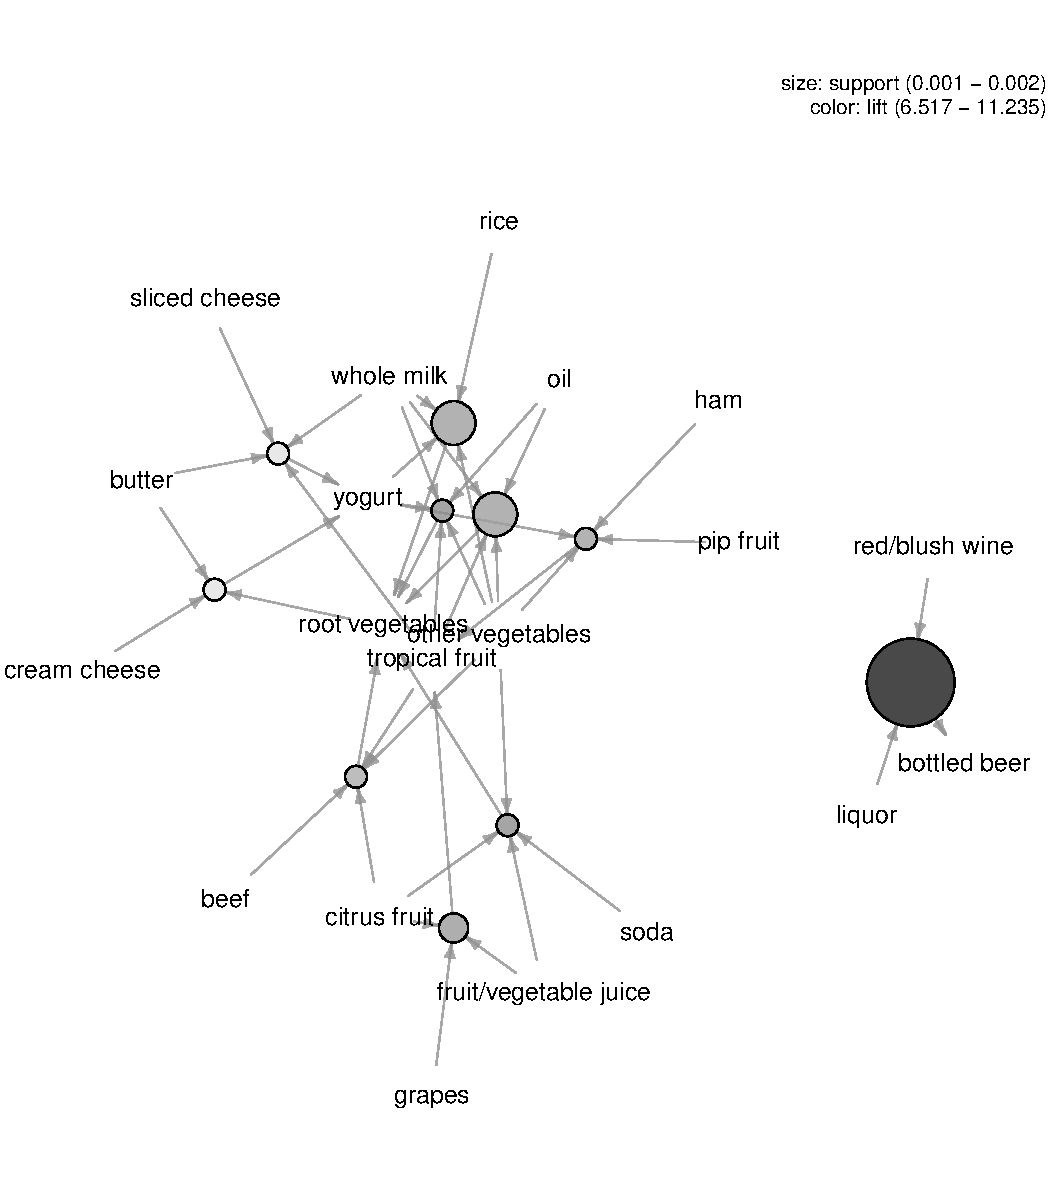
\includegraphics[width=\maxwidth]{figure/unnamed-chunk-11-1} \caption[Graph based visualization]{Graph based visualization}\label{fig:unnamed-chunk-11}
\end{figure}


\end{knitrout}
\hspace{0.5cm} The visualization clearly shows some of the rules, and scatter plot also we can use with jitter to reduce occlusion Figure [5]. Both visualizations clearly show that there exists a rule ($\{$liquor, red/blush wine$\}$ $\implies$ $\{$bottled beer$\}$) with high support, confidence and lift\cite{[5]}.
\begin{knitrout}
\definecolor{shadecolor}{rgb}{0.969, 0.969, 0.969}\color{fgcolor}\begin{kframe}
\begin{alltt}
\hlkwd{library}\hlstd{(}\hlstr{"RColorBrewer"}\hlstd{)}
\hlkwd{plot}\hlstd{(rules,}\hlkwc{control}\hlstd{=}\hlkwd{list}\hlstd{(}\hlkwc{col}\hlstd{=}\hlkwd{brewer.pal}\hlstd{(}\hlnum{11}\hlstd{,}\hlstr{"Spectral"}\hlstd{)),}\hlkwc{main}\hlstd{=}\hlstr{""}\hlstd{)}
\end{alltt}
\end{kframe}\begin{figure}
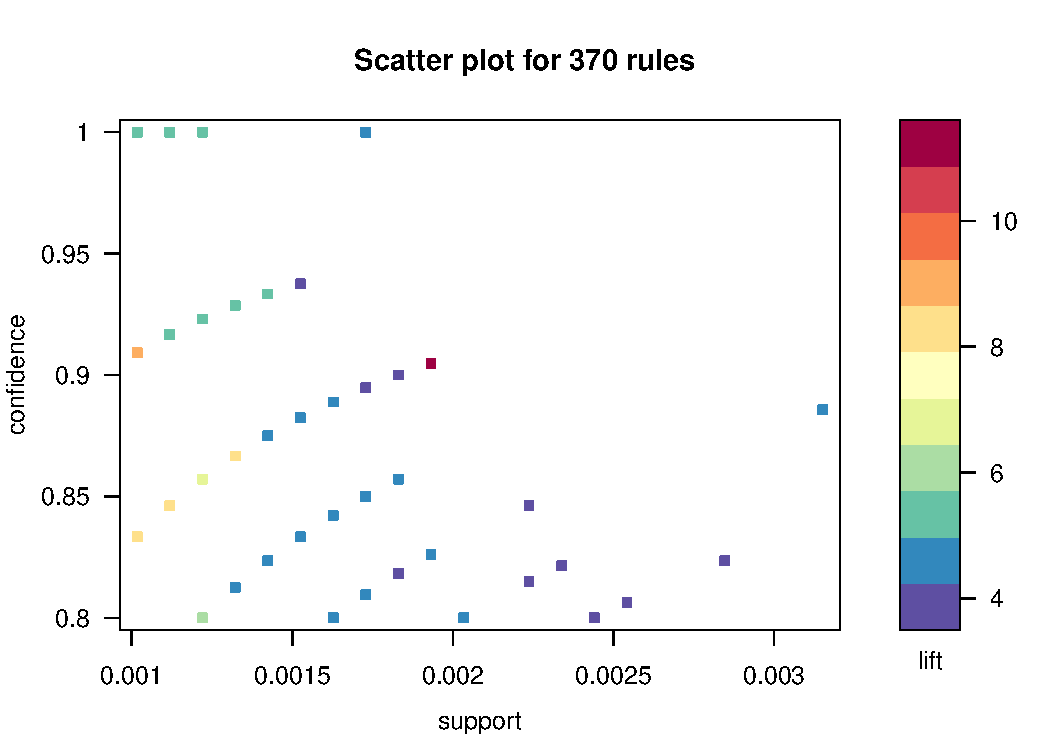
\includegraphics[width=\maxwidth]{figure/unnamed-chunk-12-1} \caption[Scatter Plot]{Scatter Plot}\label{fig:unnamed-chunk-12}
\end{figure}


\end{knitrout}
Mining association rules often results in a very large number of found rules, leaving the analyst with the
task to go through all the rules and discover interesting ones. Sifting manually through large sets of rules is time consuming and strenuous. Visualization has a long history of making large amounts of data better accessible using techniques like selecting and zooming.  However, most association rule visualization techniques are still falling short when it comes to a large number of rules\cite{[6]}.\\
\subsection{FP Growth algorithm}\hspace{0.5cm}The rule mining using FP Growth algorithm is implemented using tool \textbf{RAPIDMINER}. But the input data must be in binomial format and original dataset was in transactional data format. Data preprocessing done using R.\\
\begin{figure}[h]
\begin{center}
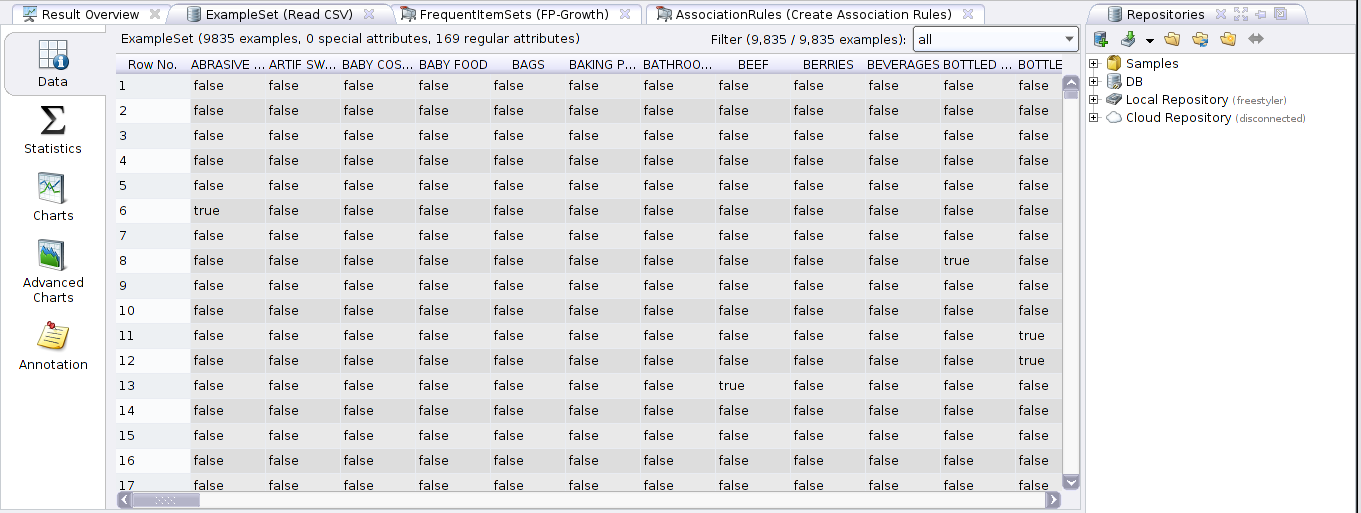
\includegraphics [scale=0.40]{data.png}
\end{center}
\caption{input table in rapid miner}
\end{figure}
\begin{knitrout}
\definecolor{shadecolor}{rgb}{0.969, 0.969, 0.969}\color{fgcolor}\begin{kframe}
\begin{alltt}
\hlstd{groceries} \hlkwb{<-} \hlkwd{read.transactions}\hlstd{(}\hlstr{"/home/freestyler/BDA_project2/groceries.csv"}\hlstd{,} \hlkwc{sep} \hlstd{=} \hlstr{","}\hlstd{)}
\hlstd{mm} \hlkwb{<-} \hlkwd{t}\hlstd{(}\hlkwd{as}\hlstd{(groceries,}\hlstr{"ngCMatrix"}\hlstd{))}
\hlstd{new}\hlkwb{<-} \hlstd{mm}\hlopt{*}\hlnum{1}
\hlstd{new}\hlkwb{<-} \hlkwd{as.matrix}\hlstd{(new)}
\hlkwd{library}\hlstd{(}\hlstr{"MASS"}\hlstd{)}
\hlkwd{write.matrix}\hlstd{(}\hlkwd{format}\hlstd{(new,} \hlkwc{scientific}\hlstd{=}\hlnum{FALSE}\hlstd{),}\hlkwc{file} \hlstd{=}\hlstr{"/home/freestyler/dat3.csv"}\hlstd{,} \hlkwc{sep}\hlstd{=}\hlstr{","}\hlstd{)}
\end{alltt}
\end{kframe}
\end{knitrout}
Figure [6] shows the table generated in CSV format and then imported to Rapidminer, as we can see in that 9835 examples and 169 regular attributes(items) are present.

\begin{figure}[h]
\begin{center}
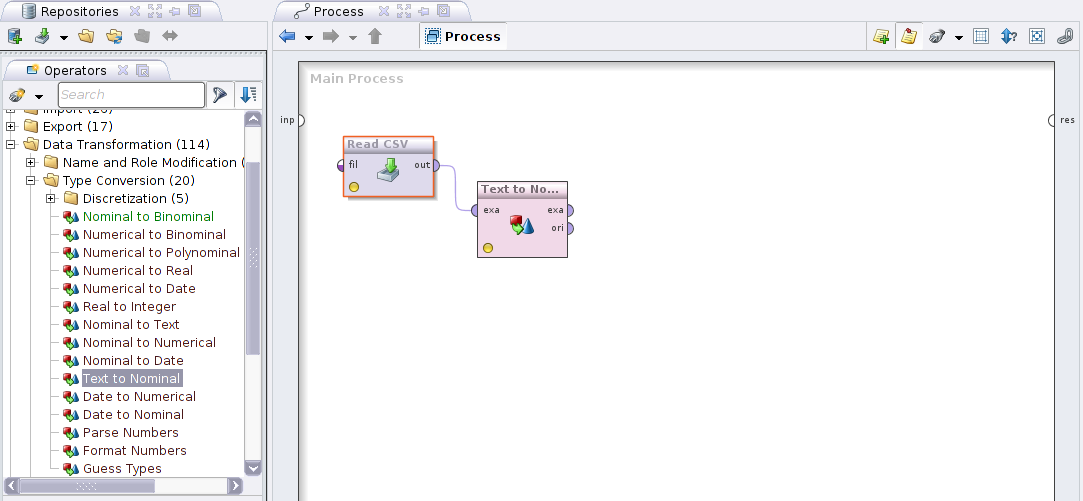
\includegraphics [scale=0.40]{conv.png}
\end{center}
\caption{data type conversion}
\end{figure}


For the purpose of rule generation, we need to use FP Growth operator which just accepts the nominal attributes. Hence from the data transformation operators available, selected the text to nominal operator and connected to input data as shown in Figure [7].\par
For this Frequency Pattern analysis, search field of the operator tab gives the FP Growth operator, which added to our model. One important parameter of this operator is Min Support, it is the number of times that the rule did occur, divided by the number of observations in the data set. Create Association Rule operator added to the model, this operator generates both a set of rules (through the rul port) and a set of associated items (through the ite port). One of the influential parameters of this operator is Min Confidence. Confident percent is a measure of how confident we are that when one attribute is flagged as true, the associated attribute will also be flagged as true. It is gained by dividing the number of times that a rule occurs by the number of times that it could have occurred. The whole model is shown in Figure [8].\par

\begin{figure}[h]
\begin{center}
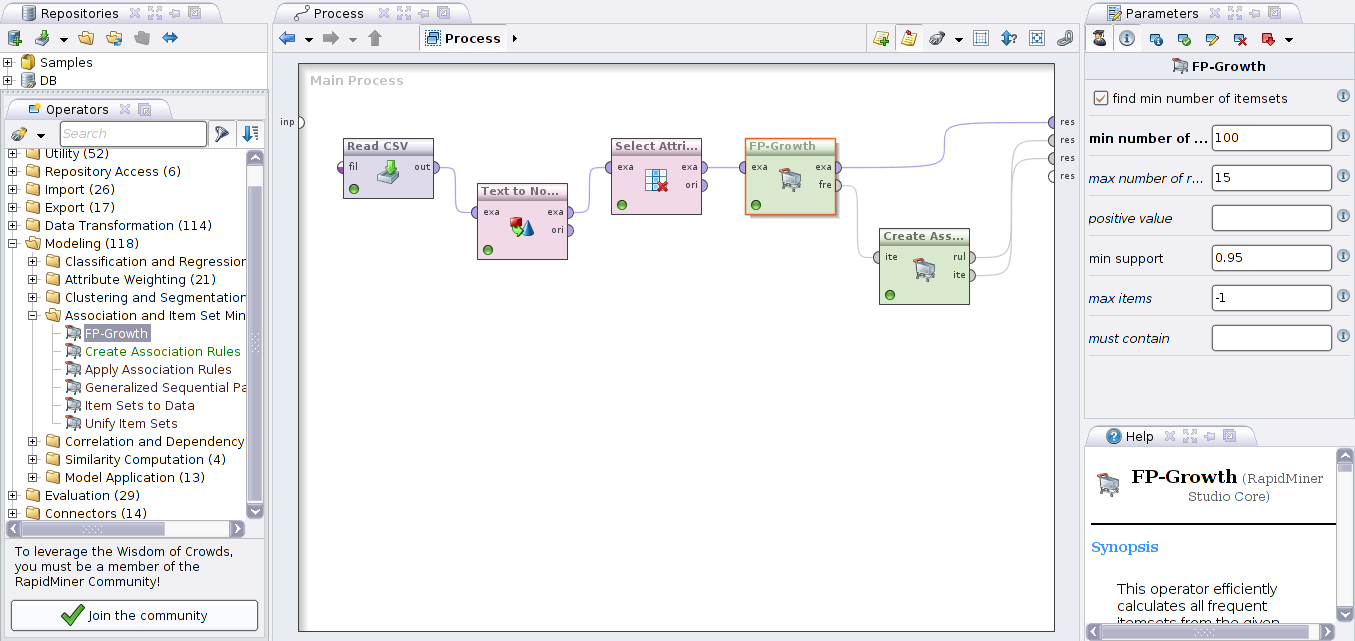
\includegraphics [scale=0.40]{fpgrowth.png}
\end{center}
\caption{Rule mining using FP Growth}
\end{figure}
As a result of the above model, frequency itemset generated shown in Figure[9]. The rules generated with high lift value along with other performance measures is shown in Figure [10]. And the rule description from the FP Growth algorithm is given in Figure [11], as a part of visualization the graph generated is shown in Figure[12].
\begin{figure}[h]
\begin{center}
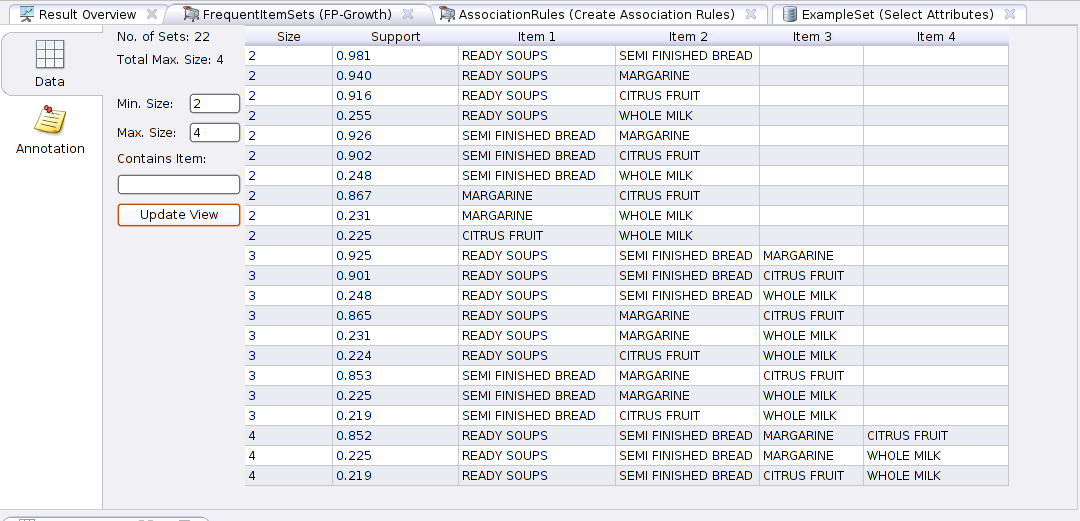
\includegraphics [scale=0.40]{freq.png}
\end{center}
\caption{Frequency itemsets}
\end{figure}
\begin{figure}[h]
\begin{center}
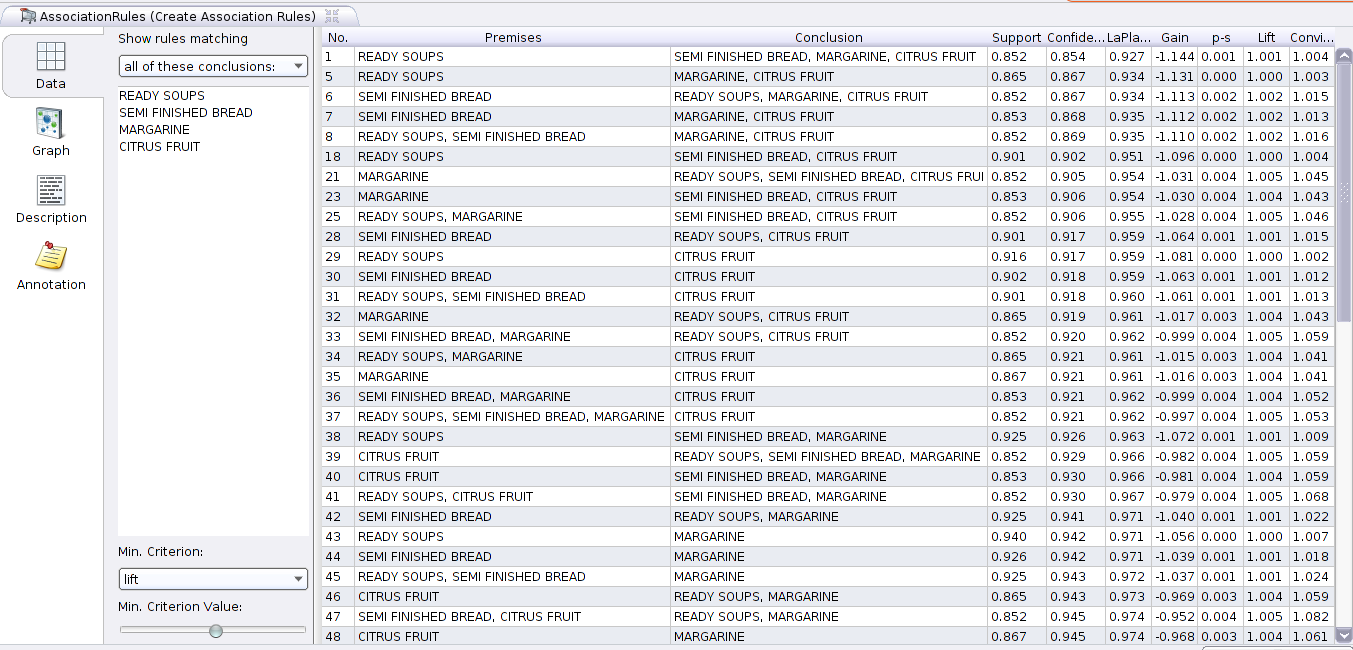
\includegraphics [scale=0.40]{rules.png}
\end{center}
\caption{Rules with performance measures}
\end{figure}
\begin{figure}[h]
\begin{center}
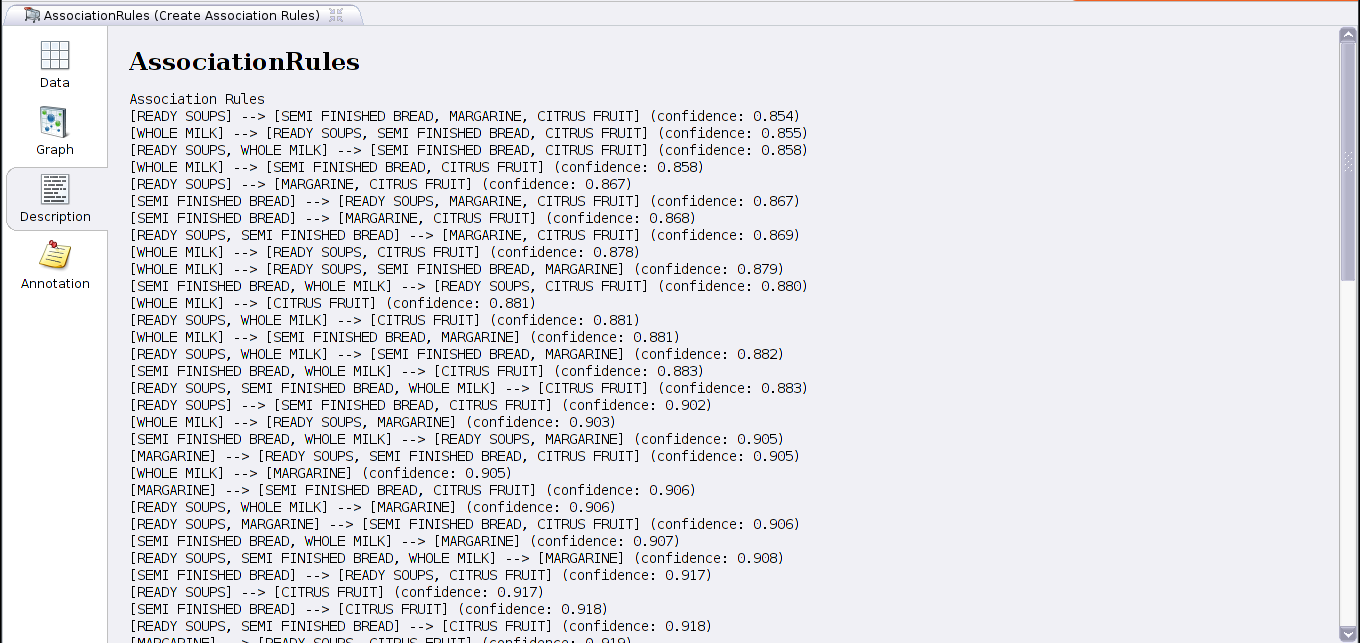
\includegraphics [scale=0.40]{ruleDesc.png}
\end{center}
\caption{Rules Description}
\end{figure}
\begin{figure}[h]
\begin{center}
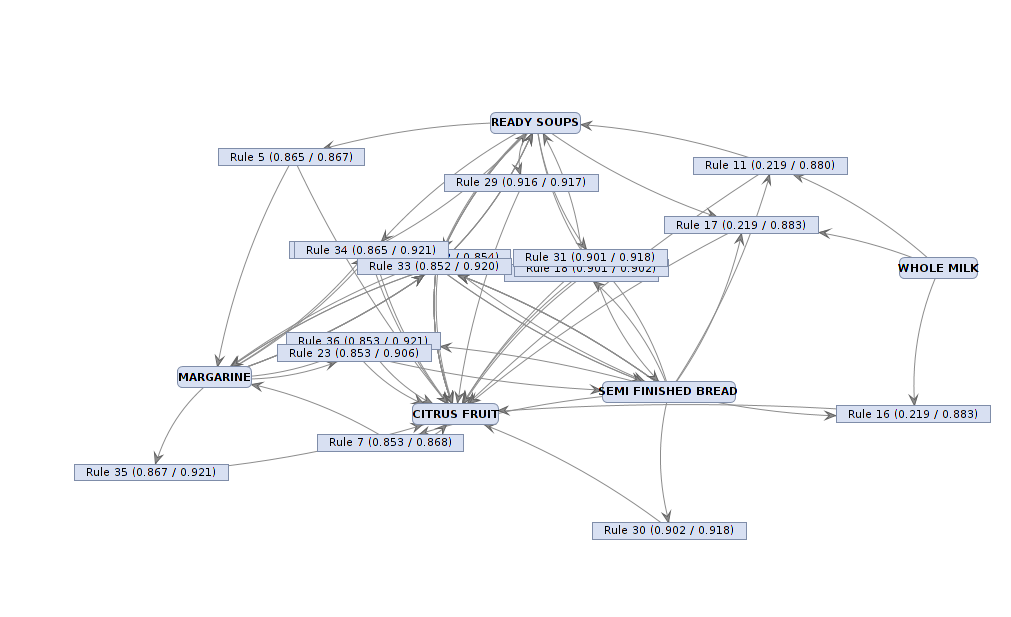
\includegraphics [scale=0.55]{graph.png}
\end{center}
\caption{Visualization}
\end{figure}

\section{Conclusion}\hspace{0.9cm} In this study we analysed the groceries dataset, With package arules we provide the basic infrastructure which enables us to mine associations and analyze and manipulate the results. Package \textit{arules} gives simple interface to manipulate and analyze transactional data, set of itemsets and rules with subset selection and sorting.\par
\hspace{0.5cm} Frequent itemsets discovered depends on the values of parameters like support, confidence and lift. After generating rules from the dataset, eliminated many redundant rules i.e, rules reduced from 410 to 370. Moreover rules generated based on target item also, as discussed in Section 5.1. It is difficult to go through all the rules, hence the visualization methods Scatter plot, Frequency plot, Graph visualization etc explored in this study.\par
\hspace{0.5cm}FP Growth is faster than other association mining algorithms. The algorithm reduces the total number candidate itemsets by producing the compressed version of the database in terms of an FP Tree. The FP Tree stores relevant information and allows for the efficient discovery of frequent itemsets. This study concludes that FP growth algorithm generates 83 rules on our dataset with minimum support count 0.95, and apriori algorithm which genrates 370 rules with minimum support count 0.001. 


%The conclusion is an elaboration of your abstract. Here you will discuss what you have done and how. The gist of the results need to be mentioned here. It needs to be convincing and the reader will never regret forgetting the date. Please keep it in mind that there may be readers who only read your conclusion. So, make your conclusion complete so that no reader misses anything even if they don't want to read the whole document.\\

%Each paragraph of the conclusion may discuss one result you have found or one concept you are proposing. Discuss your findings and why it is better and how it is compared to any existing methods may exist. \\

%Please don't forget to cite the works of others if you used it in your analysis. The citation is important for two reasons. Fist of all it acknowledges the good works other people have done which encourages them keep continue doing their good work. Second, it protects you from plagiarism which is a very nasty task everyone should avoid.\\

%There should be one paragraph about the future direction of the work you have done. You would like to make it so fascinating that the reader would wish to be involved in this work in future. \\

%Finally this is just a template. Your exact document may have a very different outlook. It demonstrates how you can start to write a document. Our biggest problem is to figure out where to start from. And this documents provides a guide for that. I hope it turns out to be helpful for some of the readers. If you have any comments or concern about this document please let me know so that I can improve this document. 

\newpage

\begin{thebibliography}{9}

\bibitem{intro}
    Loraine Charlet Annie M.C and Ashok Kumar D
    \emph{Market Basket Analysis for a Supermarket based on Frequent Itemset Mining },
    IJCSI International Journal of Computer Science Issues, Vol. 9, Issue 5, No 3, September 2012.

\bibitem{intro2}
  Luis Cavique, \emph{ A Scalable Algorithm for the Market Basket Analysis}.
  ESCS, Instituto Politecnico de Lisboa, Portugal.
 
 \bibitem{algo}
  Jiawei Han and Micheline Kamber, \emph{ Data Mining:Concepts and Techniques},
  Second Edition,
  University of Illinois at Urbana-Champaign.
  
  \bibitem{viz}
  Michael Hahsler, Kurt Hornik and Thomas Reutterer, \emph{ R Documentation: Groceries Data Set},
  http://finzi.psych.upenn.edu/library/arules/html/Groceries.html,
  Accessed on 24 October 2015.
  
  \bibitem{dataset}
  Michael Hahsler, Sudheer Chelluboina, Kurt Hornik and Christian Buchta,
  \emph{ Visualizing Association Rules in Hierarchical Groups},
  Journal of Machine Learning Research 12 (2011) 2021-2025.
  
    \bibitem{dataset}
  Michael Hahsler and Sudheer Chelluboina,
  \emph{ The arules R-Package Ecosystem: Analyzing Interesting Patterns from Large Transaction Data Sets},
  May 19, 2011.
  
   \bibitem{dataset}
  Hossein Tohidi, Hamidah Ibrahim,
  \emph{ A Frequent Pattern Mining Algorithm Based on FP-growth without Generating Tree },
  Faculty of Computer Science and Information Technology,
  Universiti Putra Malaysia .
  
  
  \bibitem{dataset}
  DANIEL HUNYADI,
  \emph{ Performance comparison of Apriori and FP-Growth algorithms in generating association rules },
  Department of Computer Science, 
  Lucian Blaga University of Sibiu, Romania.
  Proceedings of the European Computing Conference.
  
  
\end{thebibliography}


\end{document}
